\documentclass[12pt]{article}
\usepackage{graphicx}
\usepackage{amsmath}
\usepackage{bbm}
\usepackage{amsfonts}
\usepackage{amssymb}
\usepackage{float}
\usepackage{epstopdf}
\usepackage[colorlinks=true, bookmarks=true]{hyperref}
\usepackage{bibtopic,wrapfig}
\usepackage{bbding}
\usepackage{listings}
\usepackage{color} %red, green, blue, yellow, cyan, magenta, black, white
\definecolor{mygreen}{RGB}{28,172,0} % color values Red, Green, Blue
\definecolor{mylilas}{RGB}{170,55,241}

%\usepackage{refcheck}
\setcounter{MaxMatrixCols}{10}

\providecommand{\U}[1]{\protect\rule{.1in}{.1in}}
\newtheorem{theorem}{Theorem}
\newtheorem{acknowledgement}[theorem]{Acknowledgement}
\newtheorem{algorithm}[theorem]{Algorithm}
\newtheorem{condition}[theorem]{Condition}
\newtheorem{corollary}[theorem]{Corollary}
\newtheorem{definition}[theorem]{Definition}
\newtheorem{example}[theorem]{Example}
\newtheorem{lemma}[theorem]{Lemma}
\newtheorem{notation}[theorem]{Notation}
\newtheorem{proposition}[theorem]{Proposition}
\newtheorem{remark}[theorem]{Remark}
\newenvironment{proof}[1][Proof]{\textbf{#1.} }{\ \rule{0.5em}{0.5em}}
\DeclareMathOperator*{\argmin}{argmin} % thin space, limits underneath in displays

% Matlab code colors
\begin{document}
\lstset{language=Matlab,%
    %basicstyle=\color{red},
    breaklines=true,%
    morekeywords={matlab2tikz},
    keywordstyle=\color{blue},%
    morekeywords=[2]{1}, keywordstyle=[2]{\color{black}},
    identifierstyle=\color{black},%
    stringstyle=\color{mylilas},
    commentstyle=\color{mygreen},%
    showstringspaces=false,%without this there will be a symbol in the places where there is a space
    %numbers=left,%
    %numberstyle={\tiny \color{black}},% size of the numbers
    %numbersep=9pt, % this defines how far the numbers are from the text
    emph=[1]{for,end,break},emphstyle=[1]\color{red}, %some words to emphasise
    %emph=[2]{word1,word2}, emphstyle=[2]{style},
}

\begin{titlepage}

\newcommand{\HRule}{\rule{\linewidth}{0.5mm}} % Defines a new command for the horizontal lines, change thickness here

\center % Center everything on the page

%   HEADING SECTIONS

\textsc{\LARGE ORT Braude College}\\[1.5cm] % Name of your university/college
\textsc{\LARGE Department of Mathematics}\\[0.5cm] % Major heading such as course name
\textsc{\LARGE B.SC. final year project}\\[0.5cm] % Minor heading such as course title
%   TITLE SECTION
\HRule \\[0.4cm]
{ \huge \bfseries First order gradient methods}\\[0.4cm] % Title of your document
\HRule \\[1.5cm]
%   AUTHOR SECTION
\begin{minipage}{0.4\textwidth}
\begin{flushleft} \large
\emph{Author:}\\
Shira Bar-Dov % Your name
\end{flushleft}
\end{minipage}
~
\begin{minipage}{0.4\textwidth}
\begin{flushright} \large
\emph{Supervisor:} \\
Assoc. Prof. Aviv Gibali  % Supervisor's Name
\end{flushright}
\end{minipage}\\[2cm]

%   DATE SECTION
{\large \today}\\[2cm] % Date, change the \today to a set date if you want to be precise
%   LOGO SECTION

\includegraphics[scale=0.3]{Braude_Logo2.png}\\[1cm] % Include a department/university logo - this will require the graphicx package

\vfill % Fill the rest of the page with whitespace

\end{titlepage}

\newpage
{
\hypersetup{linkcolor=black}
\tableofcontents
}

\newpage
\section{Abstract}
In this project we describe and analyze different kinds of iterative first order gradient algorithms for solving optimization problems arising in image processing and support vector machines.\\
This class of methods, which can be viewed as an extension of the classical gradient algorithms, are attractive due to their simplicity and thus they adequate for solving large-scale problems even with dense matrix data. 
However, such methods are also known to converge quite slowly.\\ 
In this project we present several powerful iterative descent method for finding a local minimum of a multivariable function, that have been proven to converge faster than classical gradient algorithms. \\
Numerical experiments for image deblurring and classification problems are given. 

\newpage
\section{Introduction}
In this project we are concerned with optimization models for data fitting and data classification. Specifically, we focus on first order gradient descent methods such as ISTA- Iterative Shrinkage Thresholding Algorithm and FISTA- Fast Iterative Shrinkage Thresholding Algorithm for data fitting and a stochastic method called Pegasos for data classification.\\
Gradient descent was invented by the french mathematician Louis Augustin Cauchy in 1847. Since then, gradient descent methods kept developing, subgradients methods and stochastic subgradient methods from convex optimization were discovered during 1960-1970.  \\
Gradient descent is a first-order iterative optimization algorithm for finding the minimum of a function. 
It is a common optimization method in machine learning algorithms, which are based on a convex function.
Through an iterative process and the use of partial differential equations, gradient descent constructs a set of parameters, in order to minimize a given cost function to its local minimum.\\
Gradient descent is based on the observation that if the multivariable function $F(x)$ is defined and differentiable in a neighborhood of a point $x$ , then $F(x)$ decreases fastest if one goes from $x$ in the direction of the negative gradient of $F$ at $x$ ,$-\nabla F(x)$. 
It follows that, if 
$$x_{n+1} = x_n -\gamma \nabla F(x_n). $$
\begin{figure}[H]
\centering
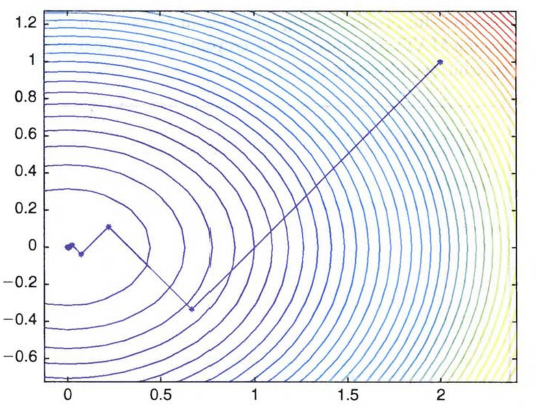
\includegraphics[scale=0.4]{gd.png}
\caption{The iterates of the gradient method along with the contour lines of the objective function}
\end{figure}
for $\gamma \in \mathbb{R}_+$ small enough, the term $\gamma \nabla F(x)$  is subtracted from $x$  because we want to move against the gradient, toward the minimum. \\
The stepsize or the learning rate $\gamma$ is a positive number that determines the size of each step in the process.
If it is too small, the process could be slow. On the other hand, if it is too large the process can skip the minimum and may not converge.
\\With this in mind, consider the unconstrained nonsmooth convex optimization problem
\begin{equation}\label{P:d4}
\min_x \{F(x) \equiv f(x) + g(x):x \in \mathbb{R}^n\}, 
\end{equation}
where $f,g$ are convex function, with $g$ possibly nonsmooth. \\
The gradient algorithm is one of the simplest methods for solving (\ref{P:d4}). It generates a sequence $\{ x_k \}$ via
$$x_0 \in \mathbb{R}^n, \;\;\; x_k = x_{k-1} -t_k (\nabla f(x_{k-1})+ \nabla g(x_{k-1})),$$
where $t_k>0$ is a suitable stepsize.\\
\\This problem arises at many different applications among them signal and image processing, optics, speech tagging and music identification. \\
When solving large-scale problems, first-order methods are often the only practical option, but the sequence ${x_k}$ converges quite slowly to a solution.\\
\\In this project, we focus on two specific models, one for data fitting with and without regulators, and one for classification. \\
Data fitting and classifying data are common tasks in machine learning.
If a parametrized model function meant to explain some phenomena is given, the goal is to adjust the numerical values for the model so that it most closely matches some data.\\
\\In data fitting problems, a classical approach to the familiar basic linear problem (\ref{P:d4}) where
$$f(x) =Ax-b,\;g(x)=0,$$
where $A\in \mathbb{R}^{m\times n},\;x \in \mathbb{R}^n,\;b\in \mathbb{R}^m,\;R(A)\;the\;column\;space\;of\;A.$\\
is the least squares, which estimate the solution by minimize the data error. In other words, if we define the error $r=Ax-b$ then we find $x=x_{ls}$ that minimize $\|r\|$. $x_{ls}$ is called least-squares approximate solution of $Ax=b$. $Ax_{ls}$ is point in $R(A)$ closest to $b$, and the projection of $b$ onto $R(A)$.
\begin{figure}[H]
\centering
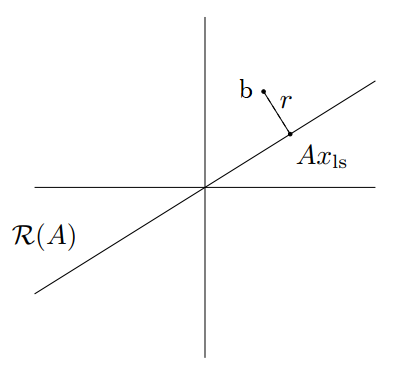
\includegraphics[scale=0.7]{ls.PNG}
\end{figure}
Note that if $b\in R(A)$ then $x_{ls}$ solves $Ax_{ls}=b$, or if $A$ is square it is invertible (nonsingular) so $x_{ls}=A^{-1}b$.\\
\\In classification problems, data points are given, and each belong to one of two or more classes. When a new point is given, the goal is to determine in which class it will be.
In support vector machines, each data point is a $p$ dimensional vector, and the goal is to determine whether it could be separated with a $p-1$ dimensional hyperplane.
Note that there are many hyperplanes that might classify the data, but the best hyperplane is the one that represents the largest separation (margin) between the two classes. Hence, the optimal hyperplane is the one that maximized the distance from it to the nearest data point on each side. 
\newpage
\section{Preliminaries}
\textbf{Convex	function:} A function $f$ is	convex	if	for	every $u,v$ in	the	domain,	and	for	every $\lambda \in [0,1]$ we have 
$$ f(\lambda u +(1-\lambda)v) \leq \lambda f(u) + (1-\lambda)f(v).$$
In	general, the necessary condition for $x$ to be a minimum for the function $f$ is $\nabla f(x)=0$. 
For	convex functions, this is both necessary and sufficient.\\
\begin{figure}[H]
\centering
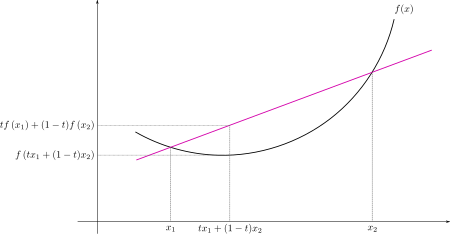
\includegraphics[scale=0.5]{convex.png}
\end{figure}
Geometrically, the inequality in the definition means the graph of $f$ between $u$ and $v$ is below the segment which joins the points $(u,f(u))$ and $(v,f(v))$.\\
%%%%%%%%%%%%%%%%%%%%%%%%%%%%%%%%%%%%
\\\textbf{$l_1$ Norm:} $l_1$ Norm is the sum of the magnitudes of the vectors in a space. A vector norm defined for a vector $\Vec{x}=(x_1,...,x_n)$ as $\|\Vec{x}\|_1 = \sum_{i=1}^{n} |x_i|$.\\
%%%%%%%%%%%%%%%%%%%%%%%%%%%%%%%%%%%%
\\\textbf{Dense matrix:} A matrix in which most of the elements are nonzero.\\
%%%%%%%%%%%%%%%%%%%%%%%%%%%%%%%%%%%%
\\\textbf{Lipschitz continuous gradient:} A  function $f$ that uphold 
$$\| \nabla f(x) - \nabla f(y) \| \leq L(f) \|x-y\| \;\;\;for \;every\; x,y \in \mathbb{R}^n ,$$
where $\| \cdot \|$ denotes the standard Euclidean norm and $L(f) > 0$ is the Lipschitz constant of $\nabla f$.\\
%%%%%%%%%%%%%%%%%%%%%%%%%%%%%%%%%%
\\\textbf{Hyperplane:} A hyperplane in an $n$ dimensional Euclidean space, is a flat  $n-1$ dimensional subset of that space that divides the space into two disconnected parts.\\
%%%%%%%%%%%%%%%%%%%%%%%%%%%%%%%%%%
\\\textbf{Inner product:} The inner product of two vectors $\vec{a} = (a_1, a_2,..., a_n)$ and $\vec{b} = (b_1, b_2,..., b_n)$ is defined as:
$$a \cdot b = a^T b =\sum_{i=1}^{n}a_i b_i = a_1b_1+a_2b_2+...+a_n b_n.$$
%%%%%%%%%%%%%%%%%%%%%%%%%%%%%%%%%%
\\\textbf{Gradient:} The gradient of a scalar multivariable function $f(x_1, x_2,...,x_n)$ is denoted $\nabla f$, packages all its partial derivative information into a vector: $\nabla f(\vec{x}) = (\frac{\partial{f}}{\partial{x_1}},\frac{\partial{f}}{\partial{x_2}},...,\frac{\partial{f}}{\partial{x_n}})$.\\
%%%%%%%%%%%%%%%%%%%%%%%%%%%%%%%%%%%%
\\\textbf{Smooth function:} A smooth function is a function that has derivatives of all orders everywhere in its domain.
 
\newpage
\section{Data Fitting}
In this section we discuss first order methods of gradient descent iterative algorithms, for solving linear inverse problems arising in image processing.\\
A basic linear inverse "image deblurring" problem $Ax=b$
\begin{figure}[H]
\centering
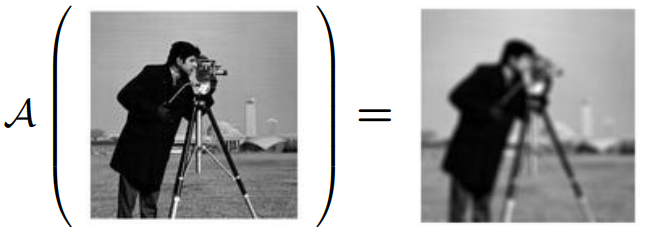
\includegraphics[scale=0.5]{df.PNG}
\end{figure}
where $A \in \mathbb{R}^{m \times n}$ represents a two-dimensional convolution blur operator, and $b \in \mathbb{R}^m$ represents the blurred image, are known. $x \in \mathbb{R}^n$ is the "true" and unknown image to be estimated, its size is assumed to be the same as that of $b$ ($n=m$). Both $x$ and $b$ are formed by stacking the columns of their corresponding two-dimensional images.\\
The blur operator or the Gaussian operator is a two-dimensional convolution operator that is used to blur images and remove detail and noise. The idea of Gaussian smoothing is to use this two-dimensional distribution as a 'point-spread' function, and this is achieved by convolution of a Gaussian mask h and the true image $x$.
\begin{figure}[H]
\centering
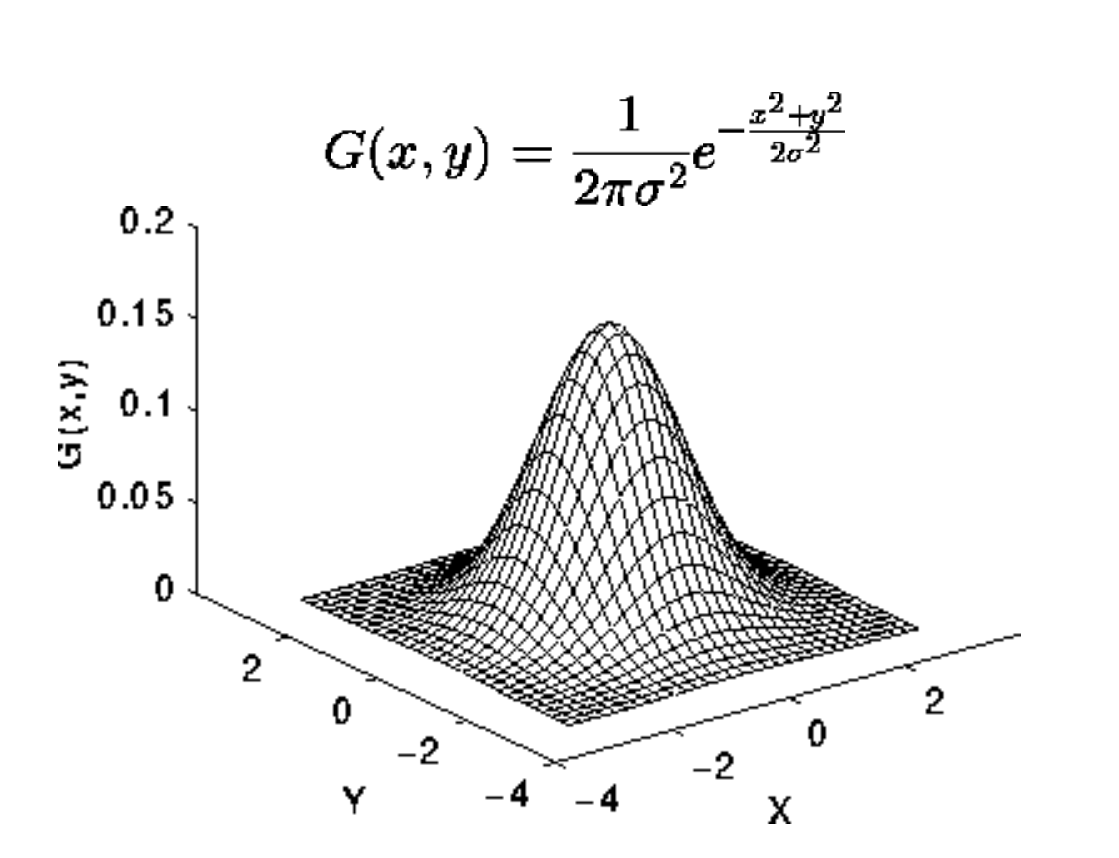
\includegraphics[scale=0.3]{gf.PNG}
\end{figure}
%%%%%%%%%%%%%%%%%%%%%%%%%%%%%%%%%%%%%%%%%%%%%%%%%%%%%%%%%%%
\subsection{ISTA}
The class of Iterative Shrinkage Thresholding Algorithms (ISTA) is an extension of the classical gradient algorithm. It is attractive due to its simplicity and thus is adequate for solving large-scale problems even with dense matrix data. \\
\\Adopting this same gradient idea to the problem formulation (\ref{P:d4}) where the following assumptions are made:\\
$ \;g: \mathbb{R}^n \rightarrow \mathbb{R}$ is a continuous convex function which is possibly nonsmooth.\\
$ \; f: \mathbb{R}^n \rightarrow \mathbb{R}$ is a continuously differentiable with Lipschitz continuous gradient $L(f)$.\\
\\Note that when $ g(x) \equiv0 $, (\ref{P:d4}) is the general unconstrained smooth convex minimization problem.\\
When $f(x) = \|Ax-b\|^2,\;g(x) \equiv \| x \|_1 $ , (\ref{P:d4}) is the $l1$ regularization problem
$$min\left\{f(x) + \lambda \|x\|_1 : x\in \mathbb{R}^n \right\}.$$
\\To calculate the Lipschitz constant of the gradient $\nabla f$ we first write $f$ as follows:
$$f(x) = \|Ax-b\|^2 = (Ax-b)^T (Ax-b)= x^T A^T Ax -x^T A^T b -b^T Ax +b^T b =$$
$$=x^T A^T Ax -(b^T Ax)^T -b^T Ax +b^T b= x^T A^T Ax -2b^T Ax +b^T b.$$
The last transaction is because the product $b^T Ax$ is a scalar product of vector $b$ and $Ax$, and therefore $(b^T Ax)^T=b^T Ax$.\\
The gradient of $\nabla f(x)$ :
$$\nabla f(x) = \nabla(x^T A^T Ax -2b^T Ax +b^T b)=(A^TA +(A^TA)^T)x-2(b^T A)^T =2A^TA x -2A^T b.$$
We define the Lipschitz continuous gradient at the preliminaries section, 
$$\| \nabla f(x) - \nabla f(y) \|= \| 2A^TA x -2A^T b-(2A^TA y -2A^T b)\| = \|2A^TA(x-y)\| \leq 2\|A^TA\| \|x-y\|.$$
The inequality is a result of the Cauchy Bunyakovsky Schwarz inequality, therefore the Lipschitz constant of the gradient is $2\|A^TA\|$. 
\begin{theorem}
Let $A$ be a symmetric $n\times n$ matrix, $\|A\|=max_j|\lambda_j|$ , where $\lambda_j$ are the eigenvalues of $A$.
\end{theorem}
\begin{proof}
The norm of a matrix is defined as 
$$\|A\| = \max_{\|u\| =1} \|Au\|.$$
Taking the singular value decomposition of the matrix $A$, we have
$$A=VDW^T,$$
where $V$ and $W$ are re orthonormal and $D$ is a diagonal matrix. Since $V$ and $W$ are orthonormal, we have $\|V\|=1$ and $\|W\|=1$. Then $\|Av\|=\|Dv\|$ for any vector $v$. Then we can maximize the norm of $Av$ by maximizing the norm of $Dv$.
By the definition of singular value decomposition, $D$ will have the singular values of $A$ on its main diagonal and will have zeros everywhere else. Let $\lambda_1,...,\lambda_n$ denote these diagonal entries so that
$$D= 
\begin{pmatrix} 
\lambda_1 & 0 & \cdots & 0 \\
0 & \lambda_2 & \cdots & 0 \\
\vdots & & \ddots & \vdots\\
0 & 0 & \cdots & \lambda_n \\
\end{pmatrix}.
$$
Taking some $v=(v_1,v_2,\cdots,v_n)^T$, the product $Dv$ takes the form
$$Dv= 
\begin{pmatrix} 
\lambda_1 v_1 \\
\vdots \\
\lambda_n v_n\\
\end{pmatrix}
.$$
Maximizing the norm of this is the same as maximizing the norm squared. Then we are trying to maximize the sum
$$S= \sum_{i=1}^{n} \lambda_i^2 v_i^2, $$
under the constraint that $v$ is a unit vector (i.e., $\sum_i v_i^2=1$). The maximum is attained by finding the largest $\lambda_i^2$ and setting its corresponding $v_i$ to 1 and then setting each other $v_j$ to 0. Then the maximum of $S$ (which is the norm squared) is the square of the absolutely largest eigenvalue of $A$. Taking the square root, we get the absolutely largest eigenvalue of $A$.
\end{proof}\\
%%%%%%%%%%%%%%%%%%%%%%%%%%%%%
\\$A^TA$ is a symmetric matrix, hence, the smallest Lipschitz constant of the gradient $ \nabla f$ is  $L(f) = 2\|A^TA\| = 2 \lambda_{max}(A^TA)$, where $\lambda_{max}$ is the maximal eigenvalue of $A^TA$.\\
%%%%%%%%%%%%%%%%%%%%%%%%%%%%%%%%%%%%%%%%%%%%%%%%%%%%%%%%%%%
\\One of the methods for solving (\ref{P:d4}) is in the class of ISTA.
The ISTA method which generates a sequence $\{x_k\}$ in this case would be:

\begin{equation}\label{P:d5}
x_0 \in \mathbb{R}^n, \;\;\; x_k = x_{k-1} -\frac{1}{L}(\nabla f(x_{k-1})+\nabla g(x_{k-1})).
\end{equation}
\\The ISTA iteration (\ref{P:d5}) can be viewed as a proximal regularization of the linearized function $f$ at $x_{k-1}$, and written equivalently as

$$x_k = \argmin_x \{f(x_{k-1}) +\langle x-x_{k-1}, \nabla f(x_{k-1}) \rangle +\frac{L}{2} \|x-x_{k-1}\|^2 + g(x)\} .$$ 
%%bounded Lipschitz function
For any $L > 0$, consider the quadratic approximation of (\ref{P:d4}) at a given point $y$:
$$Q_L (x,y) := f(y) + \langle x-y, \nabla f(y)\rangle + \frac{L}{2} \|x-y\|^2 + g(x),$$
which admits a unique minimizer
$$p_L(y) := \argmin \left\{Q_L(x,y) :x \in \mathbb{R}^n\right\}.$$
Simple Algebra shows that 
$$Q_L (x,y) := f(y) + \langle x-y, \nabla f(y)\rangle + \frac{L}{2} \langle x-y,x-y \rangle + g(x) =$$
$$= g(x) + \frac{L}{2} \langle x-y, \frac{2}{L} \nabla f(y)\rangle + \frac{L}{2} \langle x-y,x-y \rangle + f(y) =$$
$$= g(x) + \frac{L}{2} \left( \langle x-y,x-y \rangle + 2 \langle x-y, \frac{1}{L} \nabla f(y)\rangle  \right) + f(y) =$$
$$= g(x) + \frac{L}{2} \left(\langle x-y + \frac{1}{L}\nabla f(y), x-y + \frac{1}{L}\nabla f(y)\rangle -  \langle \frac{1}{L}\nabla f(y),\frac{1}{L}\nabla f(y) \rangle \right) + f(y) =$$
$$= g(x) + \frac{L}{2} \left \|x-y + \frac{1}{L}\nabla f(y)\right\|^2 - \frac{1}{2L} \left\|\nabla f(y)\right\| + f(y).$$
ignoring constant terms in y
$$p_L (y) = \argmin_{x} \left\{g(x) + \frac{L}{2} \left\| x-\left(y-\dfrac{1}{L}\nabla f(y)\right)\right\|^2\right\}.$$
Then, the gradient algorithm ISTA generates a sequence $\{x_k\}$ via

$$ x_0 \in \mathbb{R}^n,\; x_k =p_L(x_{k-1}),$$
where $L>0$ plays the role of a stepsize.\\
\\To conclude,  the basic iteration of ISTA for solving problem (\ref{P:d4}) with constant stepsize is:\\
\\\fbox{\begin{minipage}{21em}
\textbf{Input:} $L:=L(f)$- A Lipschitz constant of $\nabla f$.\\
\textbf{Initialize:} Take $x_0 \in \mathbb{R}^n$\\
\textbf{Step k:} For each $k\geq 1$ compute $$x_k = p_L(x_{k-1}).$$
\end{minipage}}
%%%%%%%%%%%%%%%%%%%%%%%%%%%%%%%%%%%%%%%%%%%%%%%%%%%%%%%%%%%
\subsection{FISTA}
A Fast Iterative Shrinkage-Thresholding Algorithm (FISTA) is an improvement of the ISTA method for solving the general problem (\ref{P:d4}).
While FISTA keeps the simplicity of ISTA, the sequence ${x_k}$ that FISTA generates converges more quickly to a solution than other gradient methods.\\
The main difference between the ISTA method and the FISTA method is that the iterative shrinkage
operator $p_L(·)$ is not employed on the previous point $x_{k-1}$, but rather at the point $y_k$, which
uses a very specific linear combination of the previous two points $x_{k−1}, x_{k−2}$. 
Obviously, the main computational effort in both ISTA and FISTA remains the same, 
because the requested additional computation for FISTA in the steps (\ref{1}) and (\ref{2}) is
clearly marginal.\\
\\The basic iteration of FISTA for solving problem (\ref{P:d4}) with constant stepsize is:\\
\\\fbox{\begin{minipage}{21em}
\textbf{Input:} $L:=L(f)$- A Lipschitz constant of $\nabla f$.\\
\textbf{Initialize:} Take $y_1=x_0 \in \mathbb{R}^n,\;t_1=1$\\
\textbf{Step k:} For each $k\geq 1$ compute 
\begin{equation}
    x_k = p_L(y_k)
\end{equation}
\begin{equation}\label{1}
    t_{k+1} = \frac{1+\sqrt{1+4t_k^2}}{2}
\end{equation}
\begin{equation}\label{2}
    y_{k+1} = x_k + \left( \frac{t_k-1}{t_{k+1}} \right)(x_k-x_{k-1}).
\end{equation}
\end{minipage}}
%%%%%%%%%%%%%%%%%%%%%%%%%%%%%%%%%%%%%%%%%%%%%%%%%%%%%%%%%%%
\subsection{Numerical experiments}
In this section we illustrate an image deblurring problem. We estimate an image $\boldsymbol{x}$ from blurred image $\boldsymbol{b}$ using the iterative gradient descent algorithms ISTA and FISTA. We compare ISTA to FISTA and show the difference between the performance of those methods.\\
Both methods were used  with a constant stepsize rule and applied once when 
\begin{equation}\label{P:e1}
f(x) = \|Ax-b\|^2, \quad g(x)=0,
\end{equation}
and once with the $l_1$ regulator when 
\begin{equation}\label{P:e2}
f(x) = \|Ax-b\|^2, \quad g(x)=\lambda \|x\|_1.
\end{equation}

\begin{figure}[H]
\centering
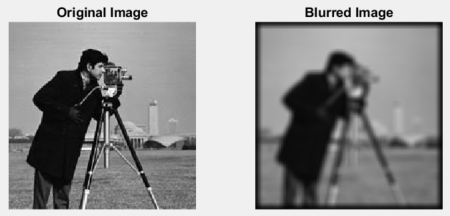
\includegraphics[scale=1]{OrgVSBlurr.png}
\caption{Deblurring of the cameraman}
\label{fig:Deb-Prob}
\end{figure}
In this example we look at the $250\times250$ cameraman image. The image went through a Gaussian blur of size $9\times9$ and standard deviation 4 (applied by the MATLAB functions conv2 and fspecial). The original and blurred images are given in Figure (\ref{fig:Deb-Prob}).\\
We tested ISTA and FISTA for solving problems (\ref{P:e1}) and (\ref{P:e2}),
where $\boldsymbol{b}$ represents the vectorized blurred image, $\boldsymbol{A}$ represents the blur operator, which is a two-dimensional convolution operator, and $\boldsymbol{x}$ represent the unknown true image.
The regularization parameter has been chosen to be $\lambda = 1$.
The Lipschitz constant was computable in this example, since the maximum eigenvalue of $A^T A$ can be calculated. \\
Iterations 5, 50, 100 and 200 of ISTA algorithm are described in Figure (\ref{fig:ISTA}).\\
Iterations 5, 50, 100 and 200 of FISTA algorithm are described in Figure (\ref{fig:FISTA}).\\
\\The peak signal to noise ratio (PSNR) for the reconstructed image is calculated, with the true image as the reference. This ratio denotes how close are we to the true image, where higher values would denote that the image is closer to the true image.\\
The function value that we want to minimize is given at those iterations, in order to track its value as it gets lower with the iterations.\\
\\\textbf{ISTA's iterations:}
\begin{figure}[H]
  \centering
    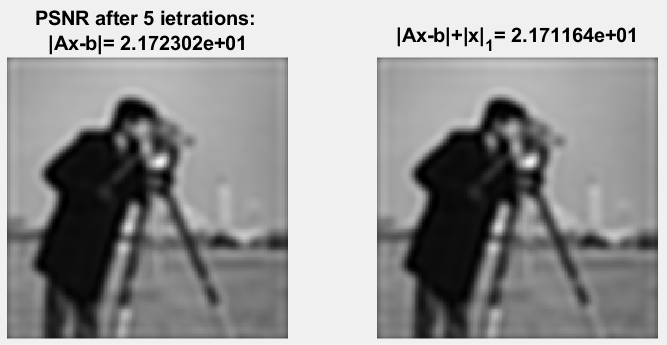
\includegraphics[scale=0.6]{Ista5.png}
 \end{figure}
\begin{figure}[H]
  \centering
    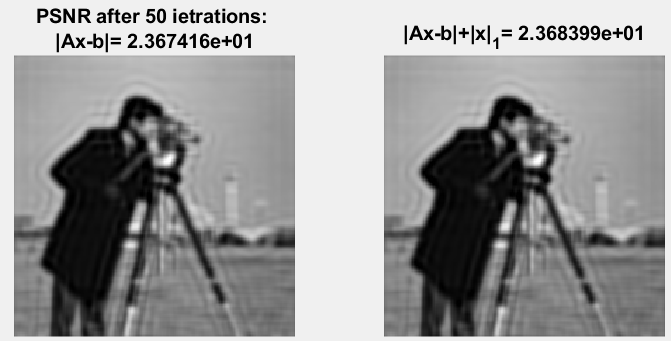
\includegraphics[scale=0.6]{Ista50.png}
 \end{figure}
 \begin{figure}[H]
    \centering
    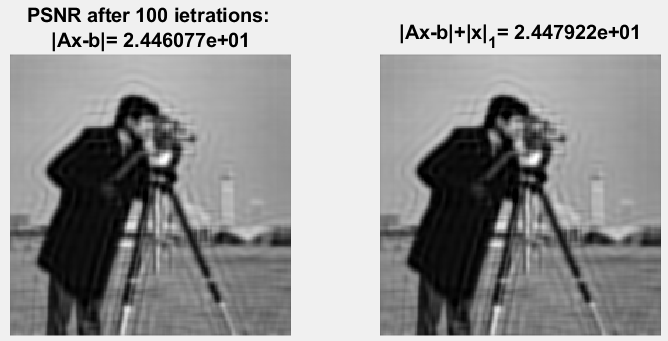
\includegraphics[scale=0.6]{Ista100.png}
\end{figure}
\begin{figure}[H]
    \centering
    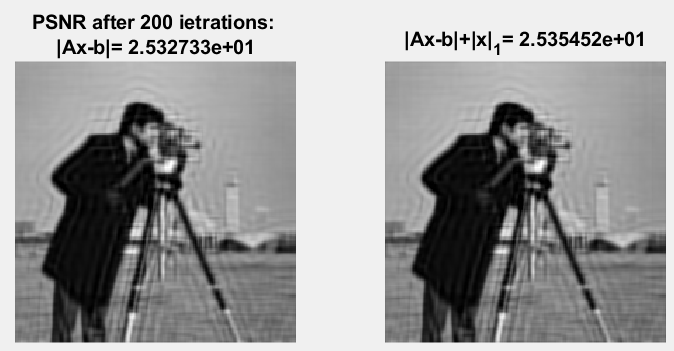
\includegraphics[scale=0.6]{Ista200.png}
  \caption{Iterations of ISTA for deblurring of the cameraman.}
  \label{fig:ISTA}
\end{figure}
\textbf{FISTA's iterations:}
\begin{figure}[H]
  \centering
    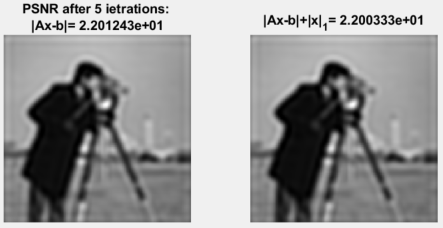
\includegraphics[scale=0.9]{Fista5.png}
 \end{figure}
\begin{figure}[H]
  \centering
    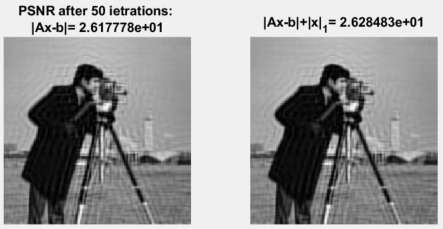
\includegraphics[scale=0.9]{Fista50.png}
 \end{figure}
 \begin{figure}[H]
    \centering
    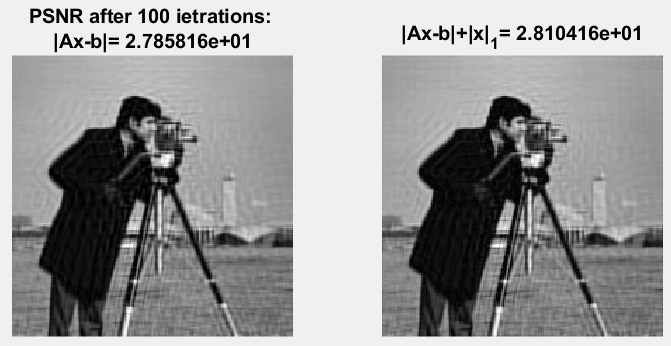
\includegraphics[scale=0.6]{Fista100.png}
\end{figure}
\begin{figure}[H]
    \centering
    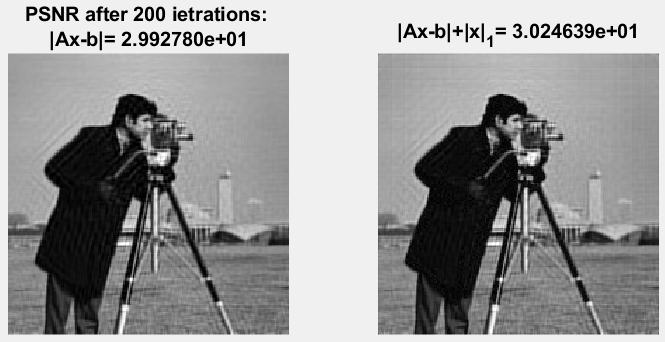
\includegraphics[scale=0.6]{Fista200.png}
  \caption{Iterations of FISTA for deblurring of the cameraman.}
  \label{fig:FISTA}
\end{figure}
\textbf{The data is summarized in the following tables:}\\

\begin{tabular}{ |p{1.5cm}|p{2.5cm}|p{2.5cm}|p{2.5cm}|p{2.5cm}|  }
 \hline
 \multicolumn{5}{|c|}{Function value of $f(x)+g(x)=\|Ax-b\|$} \\
 \hline
  & 5 iterations & 50 iterations & 100 iterations & 200 iterations\\
 \hline
 ISTA  & 3.453e+05 & 2.662e+04    & 1.292e+04   & 5.535e+03\\
 FISTA &  2.033e+05 & 2.282e+03    & 4.887e+02   & 9.660e+01\\
 \hline
\end{tabular} 
\\

\begin{tabular}{ |p{1.5cm}|p{2.5cm}|p{2.5cm}|p{2.5cm}|p{2.5cm}|  }
 \hline
 \multicolumn{5}{|c|}{Function value of $f(x)+g(x)=\|Ax-b\|+ \|x\|_1$} \\
 \hline
  & 5 iterations & 50 iterations & 100 iterations & 200 iterations\\
 \hline

 ISTA  &  5.079e+06 & 4.766e+06    & 4.752e+06   & 4.745e+06\\
 FISTA &   4.940e+06 & 4.742e+06    & 4.740e+06   & 4.739e+06\\
 \hline
\end{tabular} \\
\\It is clear that FISTA gives better results than ISTA, because the function values of FISTA are consistently lower than the function values of ISTA.\\ 
Note that the function value of FISTA after only 50 iterations is better than the function value of ISTA after 200 iterations. \\


\begin{tabular}{ |p{1.5cm}|p{2.5cm}|p{2.5cm}|p{2.5cm}|p{2.5cm}|  }
 \hline
 \multicolumn{5}{|c|}{PSNR: peak signal to noise ratio for $f(x)+g(x)=\|Ax-b\|$} \\
 \hline
  & 5 iterations & 50 iterations & 100 iterations & 200 iterations\\
 \hline
 ISTA  & 2.172+01 & 2.367+01 & 2.446+01 & 2.533+01\\
 FISTA & 2.201+01 & 2.618+01 & 2.786+01 & 2.993+01\\
 \hline
\end{tabular} 
\\

\begin{tabular}{ |p{1.5cm}|p{2.5cm}|p{2.5cm}|p{2.5cm}|p{2.5cm}|  }
 \hline
 \multicolumn{5}{|c|}{PSNR: peak signal to noise ratio for $f(x)+g(x)=\|Ax-b\|+ \|x\|_1$} \\
 \hline
  & 5 iterations & 50 iterations & 100 iterations & 200 iterations\\
 \hline
 ISTA  & 2.171+01 & 2.368+01 & 2.448+01 & 2.535+01\\
 FISTA & 2.200+01 & 2.628+01 & 2.810+01 & 3.025+01\\
 \hline
\end{tabular} \\
\\Here too, it is clear that FISTA gives better results than ISTA, because the PSNR of the FISTA method compared with the original image is consistently higher than the PSNR of the ISTA method compared with the original image.\\ 
Note that the PSNR of function $f(x)+g(x)=\|Ax-b\|+ \|x\|_1$ is consistently higher than the PSNR of function $f(x)+g(x)=\|Ax-b\|$, so we can say that the $l_1$ regulator helps the iterations to converge faster. \\
\newpage
\section{Classification}
In this section we discuss Stochastic Sub-Gradient Descent algorithms (SGD) for solving the optimization problem cast by Support Vector Machines.\\
%%%%%%%%%%%%%%%%%%%%%%%%%%%%%%%%%%%%%%%%%%%%%%%%%%%%%
SGD is a modification of the basic gradient descent algorithm, which allows us scaling these algorithms to much bigger training sets. \\
%%%%%%%%%%%%%%%%%%%%%%%%%%%%%%%%%%%%%%%%%%%%%%%%%%%%
The problem with gradient descent is that if the number of the training examples is much bigger, computing the gradient could be very expensive or even impossible because each step requires storing all the data, and calculates the derivative. 
SGD doesn't need to look at all of the training set in every single iteration, but only at a single training example. \\
Support vector machine is a linear model for classification and regression problems that constructs a hyperplane that separates the data into classes.
First, it randomly reorders the data examples, a pre-processing step which ensures that when scanning through the training set, the order of visiting the training examples would be in randomly sorted order, that speeds up the convergence.\\
Then it finds the points closest to the hyperplane from both the classes. These points are called support vectors. 
Then, the distance between the hyperplane and the support vectors is computed. This distance is called the margin.
The goal is to maximize the margin, so the hyperplane for which the margin is maximized is the optimal hyperplane.\\
The main difference between gradient descent and SGC is that in SGC the algorithm modifies the parameters a little bit for every iteration on \textbf{one} training example to fit just the specific training example a little bit better. \\
%%%%%%%%%%%%%%%%%%%%%%%%%%%%%%%%%%%%%%%%%%%
%%%%%%%%%%%%%%%%%%%%%%%%%%%%%%%%%%%%%%%%%%%%%%%
\\Formally, given a training set $S= \{(\vec{x}_i,y_i)\}_{i=1}^{m}$ where $\Vec{x}_i \in \mathbb{R}^n$ and $y_i \in \{+1, −1\}$, we would like to find the minimizer of the problem
\begin{equation}\label{P:8}
    \min_{\vec{w}} \frac{\lambda}{2}\|\vec{w}\|^2 + \frac{1}{m} \sum_{(\vec{x},y) \in S} l(\vec{w};(\vec{x},y)),
\end{equation}
where 
\begin{equation}
    l(\vec{w};(\vec{x},y))=max\{0,1-y\langle \vec{w},\vec{x} \rangle \},
\end{equation}
$\langle u,v \rangle$ denotes the standard inner product between the vectors $u$ and $v$, $\lambda$ is the regularization parameter of SVM, and $l$ is called the Loss function.\\
We denote that 
$$ f(w) = \frac{\lambda}{2}\|\vec{w}\|^2 + \frac{1}{m} \sum_{(\vec{x},y) \in S} l(\vec{w};(\vec{x},y)),$$
hence, the gradient decent iterative algorithm in this case would be:\\
$$w_{t+1} = w_t - \eta_t \nabla f(w_t), $$
where $\eta_t>0$ is called the learning rate. 
The gradient $\nabla f$ would be:
$$\nabla f(w) = \lambda \|w\| + \frac{\partial}{\partial w} max \{ 0,1-y \vec{w} \cdot\vec{x} \} ,$$
where the sub gradient is 
\begin{equation}
    \frac{\partial}{\partial w}= \left\{
  \begin{aligned}
    - y_i x_i, &\qquad& y_i \vec{w} \cdot\vec{x_i} <1, \\
    0, &\qquad& y_i \vec{w} \cdot\vec{x_i} =1, \\
    0, &\qquad& y_i \vec{w} \cdot\vec{x_i} >1, 
  \end{aligned}
  \right.
\end{equation}
if $y_i \vec{w} \cdot\vec{x_i} <1 $ than\\
\begin{equation}\label{grad}
    \qquad w_{t+1} = w_t - \eta_t (\lambda \|w_t\|  - y_i x_i  ),\\
\end{equation}
else ($y_i \vec{w} \cdot\vec{x_i} \geq1 $) than
\begin{equation}\label{grad2}
    \qquad w_{t+1} = w_t - \eta_t \lambda \|w_t\|.
\end{equation}
%%%%%%%%%%%%%%%%%%%%%%%%%%%%%%%%%%%%%%%%%%%%%%%%%%%%%%%%%%%%%%%%%%%%%%%%%%%%%%
\\Any hyperplane can be written as the set of points $\vec{x} $ satisfying $\vec{w}\cdot \vec{x}-b=0$ where $\vec{w}$ is the normal vector to the hyperplane. The following constraint were added to prevent data points from falling into the margin, for each $i$ either:\\
\indent $\vec{w} \cdot \vec{x}_i -b \geq 1$, if $ y_i=1 $ ,\\
or\\
\indent $\vec{w} \cdot \vec{x}_i -b \leq 1$, if $ y_i=-1 $ .\\
These constraints state that each data point must lie on the correct side of the margin. It could also be written as:
\begin{equation}
    y_i (\vec{w} \cdot \vec{x}_i -b) \geq 1, \;\;\; for \; all \;\; 1\leq i \leq n.
\end{equation}

\begin{figure}[H]
\centering
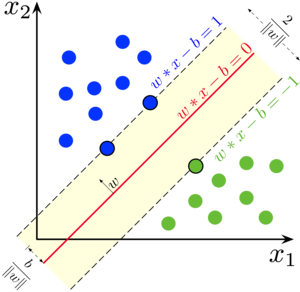
\includegraphics[scale=3]{SVM_margin.png}
\caption{Maximum-margin hyperplane and margins for an SVM trained with samples from two classes}
\end{figure}

\subsection{Pegasos}
Pegasos performs stochastic gradient descent on the primal
objective (\ref{P:8}) with a carefully chosen stepsize. Pegasos gets as input $S$ set of data examples, $\lambda$ the regularization parameter of SVM and $T$ the number of iterations.\\
%%%%%pseudo_code
\\\fbox{\begin{minipage}{20em}
\textbf{Input:} $S,\lambda,T$\\
\textbf{Initialize:} Set $w_1 =0$\\
For $t=1,2,...,T$\\
\indent Choose $i_t \in \{1,...,|S|\}$ uniformly at random.\\
\indent Set $\eta_t = \frac{1}{\lambda t}$\\
\indent If $y_{i_t} \langle w_t,x_{i_t} \rangle <1 $, then:\\
\indent \indent Set $w_{t+1} \leftarrow (1-\eta_t \lambda)w_t + \eta_t y_{i_t} x_{i_t}$\\
\indent Else (if $y_{i_t} \langle w_t,x_{i_t} \rangle \geq 1 $):\\
\indent \indent Set $w_{t+1} \leftarrow (1-\eta_t \lambda)w_t$\\
\textbf{Output:} $w_{T+1}$
\end{minipage}}\\
%%%%%%%%%%%%%%%%
\\On each iteration Pegasos operates in the following manner. Initially, it sets $w_1$ to the zero vector. On iteration $t$, it first chooses a random training example
$(x_{i_t},y_{i_t})$ by picking an index $i_t \in {1, . . . , m}$ uniformly at random. Then, it replaces the objective in (\ref{P:8}) with an approximation based on the training example $(x_{i_t} , y_{i_t})$, yielding:
$$f(w;i_t) = \frac{\lambda}{2}\|w\|^2 + l(w; (x_{i_t} , y_{i_t})). $$
The sub gradient of the above approximate objective is given by:
$$ \nabla_t = \lambda w_t - \mathbbm{1} [y_{i_t} \langle w_t, x_{i_t} \rangle < 1] y_{i_t}x_{i_t},$$
where $\mathbbm{1} [y\langle w, x \rangle < 1]$ is the indicator function which takes a value of one if its argument is true ($w$ yields non-zero loss on the example $(x, y)$), and zero otherwise. Then it updates $w_{t+1} \leftarrow w_t - \eta_t\nabla t $ using a step size of $\eta_t = \frac{1}{\lambda t}$. Note that this update can be written as:
$$w_{t+1} \leftarrow \left(1 - \frac{1}{t} \right)w_t + \eta_t \mathbbm{1}\left[y_{i_t} \langle w_t, x_{i_t} \rangle < 1\right] y_{i_t}x_{i_t}\; .$$
After $T$ iterations, the last iterate $w_{T +1}$ is returned.
\subsection{Numerical experiments}
In this section we illustrate a data classification problem. We estimate a hyperplane $w^Tx-b$ from a set of data and its labels $\{(\vec{x}_i,y_i)\}_{i=1}^{m}$ using the a built in SVM classifier in MATLAB and a stochastic gradient descent algorithm Pegasos. We compare those two algorithms and show the hyperplane each function finds.\\
%%%%%%%%%%%%%%%%%%%%%%%%%%%%%%%%%%%%%
In this example we would like to classify recipes as cupcakes or muffins. When given a new recipe, our model could determine if it's a cupcake or a muffin. We took 82 different recipes of cupcakes and muffins and normalized the data to percentage of the whole batter. Then, we chose 2 ingredients- butter and sugar that we've noticed that are different between those two types of recipes.   
\begin{figure}[H]
  \centering
    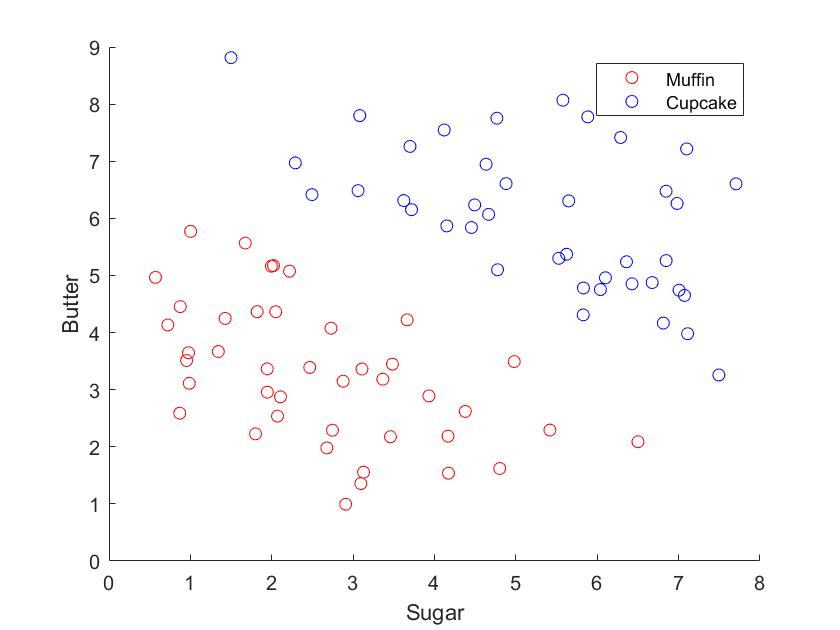
\includegraphics[scale=0.3]{sugarbutter.jpg}
 \end{figure}
As you can see muffins have little sugar and little butter and cupcakes have a lot of sugar and a lot of butter, therefore it's a good example for SVM classify.\\ 
First, the data went through the SVM classifier (applied by the MATLAB function fitcsvm), the hyperplane and the support vectors solution for this problem are given in Figure (\ref{fig:svm}).
\begin{figure}[H]
  \centering
    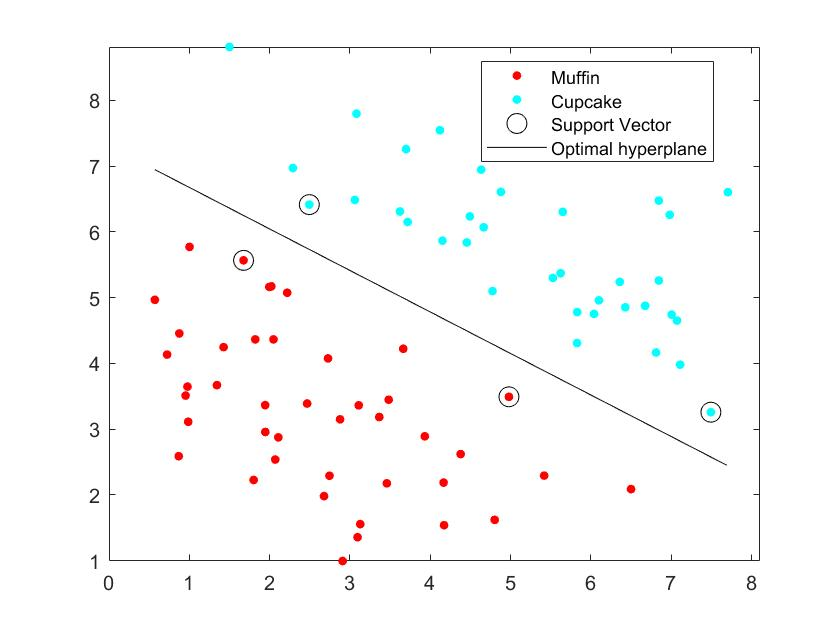
\includegraphics[scale=0.25]{SVM.jpg}
    \caption{SVM hyperplane and support vector}
    \label{fig:svm}
 \end{figure}
\textit{The hyperplane defined by SVM is $(0.93,1.47)x -10.71$.}\\
Then, we have implemented the Pegasos algorithm on MATLAB, the hyperplane and its margins are given in Figure (\ref{fig:Pegasos})
 \begin{figure}[H]
  \centering
    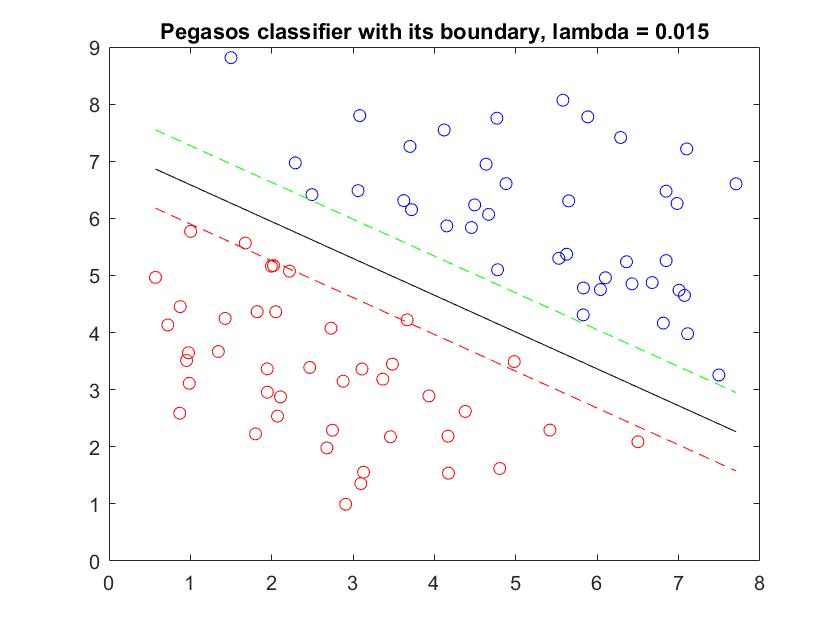
\includegraphics[scale=0.25]{Pegasos.jpg}
    \caption{Pegasos hyperplane and its margins}
    \label{fig:Pegasos}
 \end{figure}
\textit{The hyperplane defined by Pegasos is $(0.94,1.46)x -10.54$.}\\
The results we got are approximately the same as the result of the built in SVM classifier function. \\
Another interesting information is the minimized function value, because we used a stochastic method we wont see a stable descent, but stochastic steps that their general target is the minimum.

 \begin{figure}[H]
  \centering
    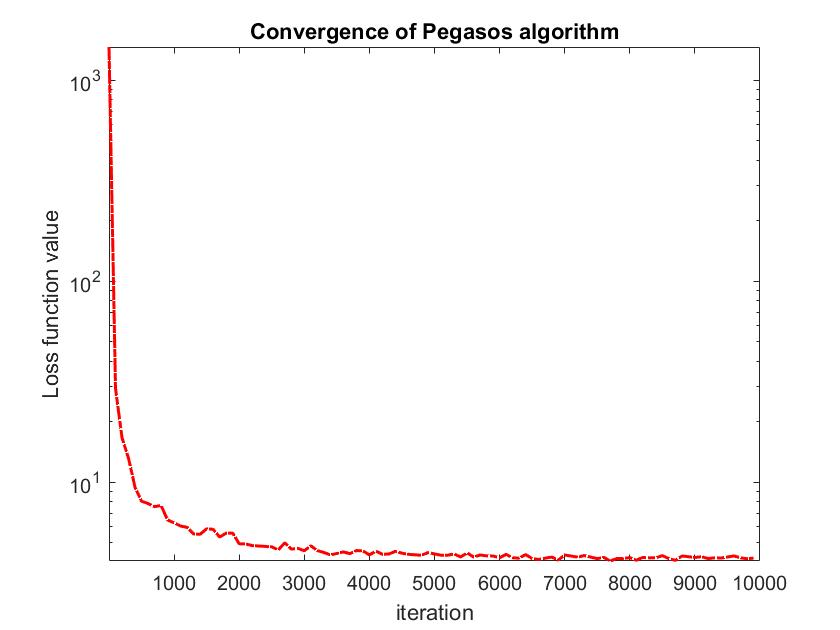
\includegraphics[scale=0.25]{ConvergeOfPegasos.jpg}
 \end{figure}
 
\newpage
\section{Conclusion}
In this project, we presented and described the gradient descent algorithm. We presented two extensions of the algorithm one at the field of data fitting and one on the field of classification. \\
We have shown that solving optimization problems is a common task in machine learning that arises at many different applications. For large-scale  problems, those methods are often the only practical option, so extending those methods with better convergence rate could yield a tremendous influence at this field.  
We have also been able to analyze and implement the data fitting methods and classification method in an extremely simple and efficient way.


\section{Acknowledgements} 
\textit{I would like to thank Assoc. Prof. Aviv Gibali for giving me the opportunity to work on this fascinating and instructive project. I would also like to thank him for the time and help he granted me to help me move forward with this project, while pushing me to be as independent as possible.}
\newpage
\section{Matlab Codes}
\subsection{Data Fitting}
\textbf{FISTA Algorithm:}
\lstinputlisting{Fista.m}
\textbf{ISTA Algorithm:}
\lstinputlisting{Ista.m}
\textbf{Image Blur:}
\lstinputlisting{Conv_Blur_Img.m}
\textbf{Elements Calculator:}
\lstinputlisting{Elements_Calc.m}
\textbf{Gradient step:}
\lstinputlisting{GradStep.m}
\textbf{Gradient step with norm1:}
\lstinputlisting{GradX1Step.m}
\textbf{Show image in current iteration:}
\lstinputlisting{Img_Per_Iter.m}
\textbf{Value of function in current iteration:}
\lstinputlisting{Fi.m}
\subsection{Classification}
\textbf{main function SVM VS Pegasos:}
\lstinputlisting{SVM_VS_Pegasos.m}
\textbf{SVM solver:}
\lstinputlisting{SVM_solver.m}
\textbf{Pegasos solver:}
\lstinputlisting{Pegasos_solver.m}
\newpage
\begin{thebibliography}{99}

\bibitem{BC1} Shalev-Shwartz, Shai, et al. "Pegasos: Primal estimated sub-gradient solver for svm." Mathematical programming 127.1 (2011): 3-30.
\bibitem{BC2} Beck, Amir, and Marc Teboulle. "A fast iterative shrinkage-thresholding algorithm for linear inverse problems." SIAM journal on imaging sciences 2.1 (2009): 183-202.
\bibitem{BC5} Beck, Amir. Introduction to nonlinear optimization: Theory, algorithms, and applications with MATLAB. Vol. 19. Siam, 2014.
\bibitem{BC3} \textcolor{blue}{https://see.stanford.edu/materials/lsoeldsee263/05-ls.pdf}
\bibitem{BC4} \textcolor{blue}{https://homepages.inf.ed.ac.uk/rbf/HIPR2/gsmooth.htm}

\end{thebibliography}

\end{document}
